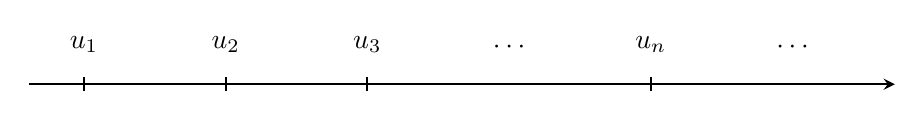
\begin{tikzpicture}[>=stealth]
    % Mũi tên biểu diễn thứ tự các số hạng của dãy số.
    \draw[->, thick] (0, 0) -- (11, 0);

    \foreach \x/\term in {0.7/u_1, 2.5/u_2, 4.3/u_3, 7.9/u_n} {
        \draw[thick] (\x, -0.09) -- (\x, 0.09)
            node[above=5pt] {$\term$};
    }

    \node[above=5pt] at (6.1, 0.09) {$\cdots$};
    \node[above=5pt] at (9.7, 0.09) {$\cdots$};
\end{tikzpicture}
